\chapter{Estado del Arte} \label{chap:estadodelarte}


En este capítulo vamos a describir las diversas investigaciones y trabajos realizados con imágenes satelitales hasta la fecha. Se pondrá a disposición del lector como se utilizaron técnicas de  Computer Vision y Machine Learning sobre imágenes satelitales.


\section{Aplicaciones en el ámbito espacial}\label{sec:estadodelacuestion}

Las aplicaciones de visión artificial en el ámbito espacial son cada ves mas utilizadas, desde el estudio de un área determinada hasta implementaciones echas a bordo de un satélite artificial. Este avance se dio gracias a diversos factores en el campo de la informática; en primer lugar la creciente capacidad de computo, con procesadores de mayor rendimiento y el auge de las GPU (unidad de procesamiento grafico). En segundo lugar la aparición de algoritmos y frameworks mas eficiente en el uso de reconocimiento de patrones; de los que podemos nombrar el uso de \ac{cnn}. 

Otro factor que no podemos dejar de nombrar son la aparición de UAVs, esto permitió utilizar Computer Vision sobre imágenes de mayor tamaño. La presencia en el mercado de pequeños UAVs de bajo costo con capacidad para portar pequeñas cámaras de vídeo de alta resolución y de realizar despegue vertical con posibilidad de movimiento en cualquier dirección del espacio, hace posible abordar nuevos retos en el campo de la detección y seguimiento de determinadas situaciones de la realidad \citep{Lanillos}.

Actualmente en el campo de reconocimiento de patrones sobre imágenes satelitales se pude ver que la mayoría de los trabajos que se realizaron en el área espacial han sido aplicado en tierra; gran parte de estos trabajos se basan en estudiar las característica del terreno. Estas aplicaciones son cada vez mas explotada no solo por agencias espaciales sino por entidades educativas, publicas y privadas. 

Para empezar vamos a comenzar citando el siguiente trabajo realizado por \citep{Cheang}; en este articulo se describe el uso de técnicas de reconocimiento de patrones usando aprendizaje supervisado. El método para la extracción y clasificación de los datos utilizado se baso en dos enfoques; por un lado se utilizaron técnicas de \textit{sliding window} para la obtención de regiones candidatas, por otro se aplicaron redes neuronales profundas, \ac{dl}, método muy utilizado para el reconocimiento de objeto en una imagen. Otro ejemplo encontrado en la literatura aplicando  \textit{aprendizaje no supervisado} es para la clasificación del uso de la tierra a partir de imágenes satelitales multi-temporales, en este paper \citep{pnn}, se utilizo imágenes del satélite LANSAT y SPOT usando redes neuronales probabilística, estas técnicas realizan un agrupamiento de datos, \textit{clusters}, y realizan la clasificación creando las fronteras entre los diferentes \textit{clusters} de datos para su posterior reconocimiento.

En el blog titulado \textit{Una imagen vale más que mil palabras}, los autores destacan el beneficio de aplicar procesamiento en imágenes para la toma de decisiones que agregan valor a su negocio. En este articulo describen la posibilidad de conocer el historial de inundaciones de una region rural aplicando técnicas \ac{ml} sobre imágenes satelitales\footnote{Fuente:http://www.7puentes.com/blog/2017/12/11/agtech-imagenes-satelitales-una-imagen-vale-mas-que-mil-palabras/}.

El uso de \ac{va} permite crear mapas urbanos a partir de imágenes satelitales como menciona en el articulo \citep{detectionHOG}; en el mismo usa \ac{va} para crearon mapas urbanos que determinan cambios temporales en una determinada región geográfica. En este trabajo los autores proponen dos módulos para el desarrollo; por un lado usar \textit{HOG}, histograma de gradientes orientados, para la extracción de características en la imagen y \textit{Local binary patterns (LBP)}, patrones binarios locales, como método descriptor de característica; por ultimo para clasifica la imagen utilizaron técnicas SVM (ver:\ref{sub:svm}). 

\cite{usman} en su articulo describe la extracción de características de una imagen satelital aplicando métodos de  detección de bordes, \textit{edges proposal}, para el 
reconocimiento de límites catastrales.

Como podemos se puede observar en los trabajos citados anteriormente, son diversas las investigaciones realizadas sobre imágenes satelitales utilizando algoritmos entrenados para reconocer patrones de interés. En el área espacial uno de los principales problemas es la limitación de energía, esto hace que el poder de computo sea mucho menor en relación a lo que podemos utilizar en tierra, por este motivo son mucho menor los ejemplos que podemos encontrar en la literatura. Sin embargo en la actualidad existen diferentes aplicaciones que están siendo utilizadas usando este tipo de técnicas de las cuales nombraremos a continuación.

Unos de los ejemplos destacados de investigaciones en\ac{va} en vuelo es el realizado por el \textit{Dr.Tweddle} que en su trabajo titulado, \textit{Computer Vision Based Navigation for Spacecraft Proximity Operations}, estudia y detalla el uso de \ac{va} para realizar una navegación autónoma en satélites. En esta tesis destaca el proyecto de un Nanosatélite, CubeSat, de la \ac{nasa} llamado , Synchronize Position Hold Engage and Reorient Experimental Satellite (\textit{SPHERES}), que dispone de un modo experimental del uso de tecnología de visión artificial, en este paper destaca la ventaja que nos pude dar del uso de \ac{va} en relación a otra tecnología de sensado \citep{Brent}.

En la actualidad existen aplicaciones desarrolladas que utilizan algoritmos de \ac{va} en un satélite artificial; la mayoría de estas aplicaciones utilizan técnicas orientadas al aprendizaje autónomo, esto se debe a las grandes distancias que existen entre la tierra y el espacio es por esto que es necesario lograr mayor autonomía en la toma de decisiones; un ejemplo de lo mencionado es el \textit{Mars Rover}, robot desarrollado para la exploración de la superficie de Marte. El \textit{Mars Rover} crea mapas de entorno de la superficie para determinar su ubicación y predecir los diferentes obstáculos que hay en su entorno \citep{RoverMars}. Este robot utiliza  diversas cámaras que aplicando técnicas de \ac{va}  permite crear mapas del entorno y realizar la predicciones de su ruta. De la misma manera el trabajo realizados  por \ac{nasa}  destaca el uso de reconocimiento de patrones en un robot por medio de diferentes cámaras que captan la profundidad y posición del objeto\footnote{Fuente: 
http://blog.infaimon.com/robots-guiados-por-vision-artificial-para-el-espacio-robos-guiados-por-visao-artificial-para-o-espaco/}. En el informe se menciona el uso de \ac{va} para brindar soporte a los astronauta en la Estación Espacial Internacional (ISS). 

Siguiendo la misma linea de investigación podemos nombrar el proyecto \textit{Docking and Capture of Satellites through computer vision}, ASIROV: Acoplamiento y Agarre de Satélites mediante Sistemas Robóticos basado en Visión \footnote{Fuente: https://goo.gl/w7iayv}, desarrollado para atracar y capturar satélites espaciales; este sistema se basa  en tecnologías de \ac{va} para guiar de forma autónoma un vehículo espacial.


Usar técnicas de \ac{va} implica lograr que el satélite tenga mayor autonomía, en el articulo realizado por \cite{Kouyama}, aplica esta tecnología para determinar la actitud y órbita del satélite basado en los datos adquiridos por los sensores del mismo; en el articulo los autores describen que para pequeños satélites,CubeSat, tienen una carga útil limitada y sus actitudes a veces son difíciles de determinar a partir de los pocos sensores que contiene a bordo por sí solos. Estas actitudes incorrectas conducen a proyecciones y mediciones inexactas que requieren corrección de pos-procesamiento en tierra. En el estudio proponen un esquema automatizado y robusto que deriva la actitud del satélite a partir de sus imágenes de observación y de la posición de satélite conocida, combinando características de tierra de una imagen observada y de imágenes registradas. El esquema combina algoritmos de \ac{va} (es decir, detección de características y validaciones robustas) y restricciones geométricas de la observación por satélite.

\cite{Huggins} en su trabajo titulado \textit{Computer Vision Localization Based on Pseudo-Satellites} propone usar técnicas de \ac{va} para la localización y orientación de un CubeSat para complementar la navegación, el estudio se enfoca en  aumentar la capacidad de los GPS utilizando \ac{va}. El autor siguiere crear una red de nodos en el cual un grupo de nodos poseen GPS para calcular su posición y el otro grupo a partir del uso de la posición de la cámara y usando técnicas de  \ac{va}  utilizar la posición del primer grupo para calcular la suya intercambiando información de los datos y calculando la distancia y orientación de la cámara \citep{Huggins}.

Como vimos existen en la actualidad estudios y aplicaciones realizadas ya sea en vuelo o en tierra que utilizan algoritmos de reconocimiento de patrones, por lo que la tendencia vista en los últimos tiempo es muy alentadora y nos abre una nueva forma de mirar al espacio y enfocar nuestro desarrollo a esta área, como podemos ver en el gráfico siguiente \ref{Fig: scopus1}. 

\begin{figure}[h]
 \centering
  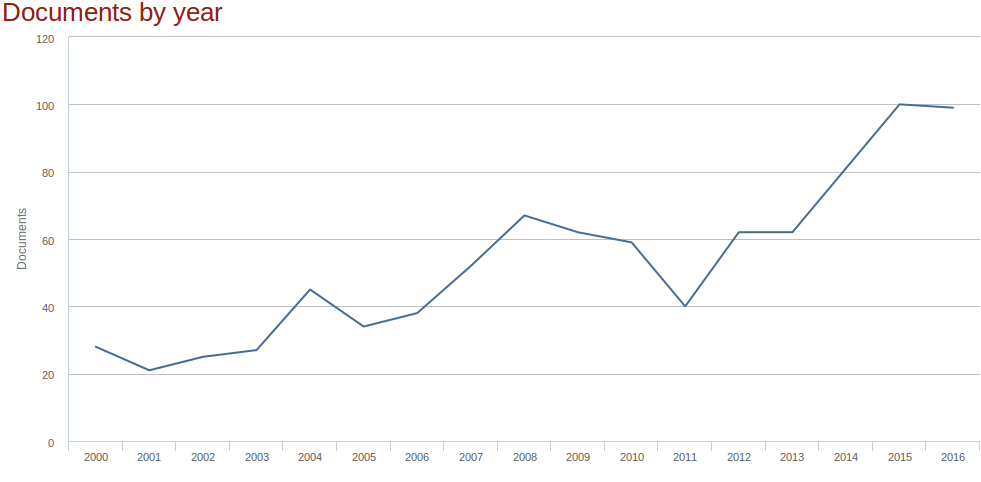
\includegraphics[height=7cm,keepaspectratio=true,clip=true]{imagenes/Logos/scopus.png}
  \caption{Extraído de Scopus.com}
	\label{Fig: scopus1}
\end{figure}
Los datos que muestran la siguiente figura \ref{Fig: scopus2} han sido relevados desde el año 2000 hasta la fecha.

\begin{figure}[h]
 \centering
  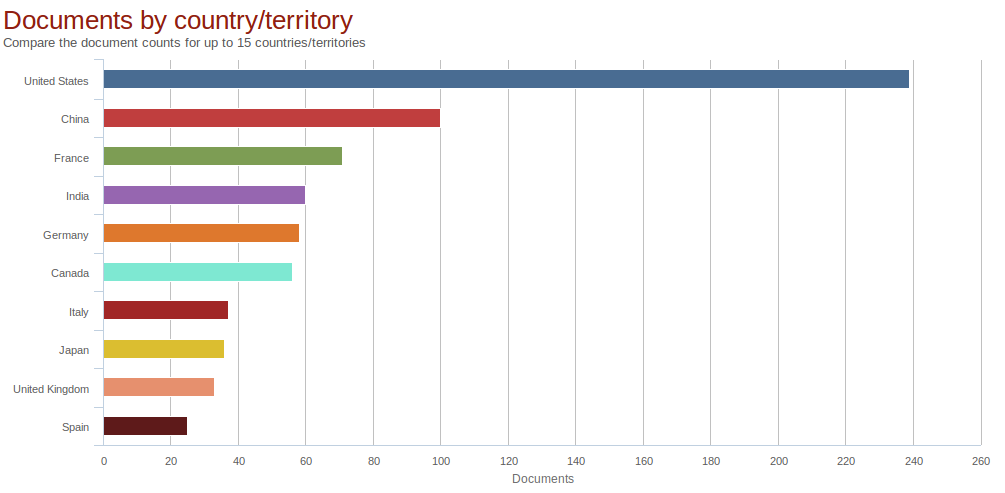
\includegraphics[height=7cm,keepaspectratio=true,clip=true]{imagenes/Logos/scopus2.png}
  \caption{Extraído de Scopus.com}
	\label{Fig: scopus2}
\end{figure}


